\documentclass{article}
\usepackage{amsmath}
\usepackage{amssymb}
\usepackage{hyperref}
\usepackage[margin=1in]{geometry}
\usepackage{graphicx}
\begin{document}
\noindent Luke Bouma, \today.

\begin{align}
Q'_{\star/p} &= Q_0' (P_\mathrm{tide})^\alpha (M)^\beta (M')^\gamma 
(P_\mathrm{spin})^\delta
\label{eq:dissipation_model} \\
Q'_{\star/p} &= 
\begin{cases}
Q_\mathrm{eq}' (P_\mathrm{tide})^{\alpha_\mathrm{eq}} \quad 
&\mathrm{if}\,|P_\mathrm{tide}|<2P_\mathrm{spin}\\
Q_\mathrm{inr}' (P_\mathrm{tide})^{\alpha_\mathrm{inr}} \quad 
&\mathrm{if}\,|P_\mathrm{tide}|\geq2 P_\mathrm{spin}
\end{cases}
\end{align}

\section{MESA stellar evolution grid}	

\texttt{POET} computes the orbital evolution of a system with a single star and 
a single planet under the influence of tides.
The tidal dissipation rate of both the star and the planet depends on the
spin period of the body damping the tidal wave 
(Eq.~\protect\ref{eq:dissipation_model}).
To assign a dissipation rate, we thus need a prescription for the angular 
momentum evolution of both the star and planet.

As the star evolves, its convective envelope loses angular momentum to 
a wind through magnetic braking (Schatzman 1962). We write this loss rate as 
Eq.~XX. In addition, the star's radiative core and convective envelopes 
exchange angular momentum (Eq.~YY). In Eq.~YY $\tau_c$ is the coupling timescale 
at which the core and envelope are driven to solid-body rotation. 

To find the time-evolution of the stellar quantities in 
Eqs.~XX and~YY, namely 
$R_\star(t),I_\mathrm{rad}(t),I_\mathrm{conv}(t),R_\mathrm{rad}(t),$ 
and $M_\mathrm{rad}(t)$, we compute stellar evolutionary tracks using 
\texttt{MESA} (Paxton et al. 2011, 2013, 2015).
We specifically follow the work of `\texttt{MESA} Isochrones \& Stellar Tracks' 
(MIST)\footnote{Currently hosted at 
\url{http://waps.cfa.harvard.edu/MIST/index.html}}, a project 
that has built and tested large grids of single-star 
evolution models across all evolutionary phases, for a wide range of masses and 
metallicities (Dotter 2016, Choi et al. 2016).

In nearly all cases, we adopt the same physics as Choi et al. 2016, hereafter 
C+16.
We downloaded the \texttt{MESA} input files (\texttt{inlists}) from the MIST 
website\footnote{\url{http://waps.cfa.harvard.edu/MIST/data/tarballs_v1.0/MESA_files.tar.gz},
\texttt{inlists} retrieved 2016-09-20.} and, subject to minor modifications, 
directly used them to compute stellar evolutionary tracks 
across our desired parameter space.
That parameter space is defined as:
\begin{align}
0.4 &\leq M_\star / M_\odot \leq 1.2\quad (0.1M_\odot\ \mathrm{spaced}) \\
-1 &\leq \mathrm{[Z/H]} \leq 0.5\quad (0.25\mathrm{dex\ spaced}),
\end{align}
where the grid resolution is primarily limited by convenience (we will 
interpolate between these grids to match them with measured masses and 
metallicities of actual stars).
We begin each stellar model in its pre-main sequence\footnote{``Uniform 
composition, $T_c=5\times10^5\,\mathrm{K}$ so no nuclear burning, and uniform 
contraction for enough luminosity to make it fully convective'' 
(\url{http://mesa.sourceforge.net/star_job_defaults.html})}, follow its 
evolution
through its main sequence, and halt it once its He core-mass reaches 
$0.1M_\odot$ (this is often when the star is older than the age of the 
universe, but it is computationally cheap and convenient in later 
interpolation).


\subsection{Adopted physics}
Table 1 of C+16 summarizes the physics behind our stellar evolution models 
(reproduced for reference as Fig.~\ref{fig:table1_C16}).
We replicate these assumptions exactly except for two points, both detailed 
below: \textit{i)} the solar abundance scale, and \textit{ii)} the specifics of 
transitions between boundary conditions as a function of stellar mass.


\subsubsection{Fine-tuned solar abundance scale}
\begin{figure}[t]
	\centering
	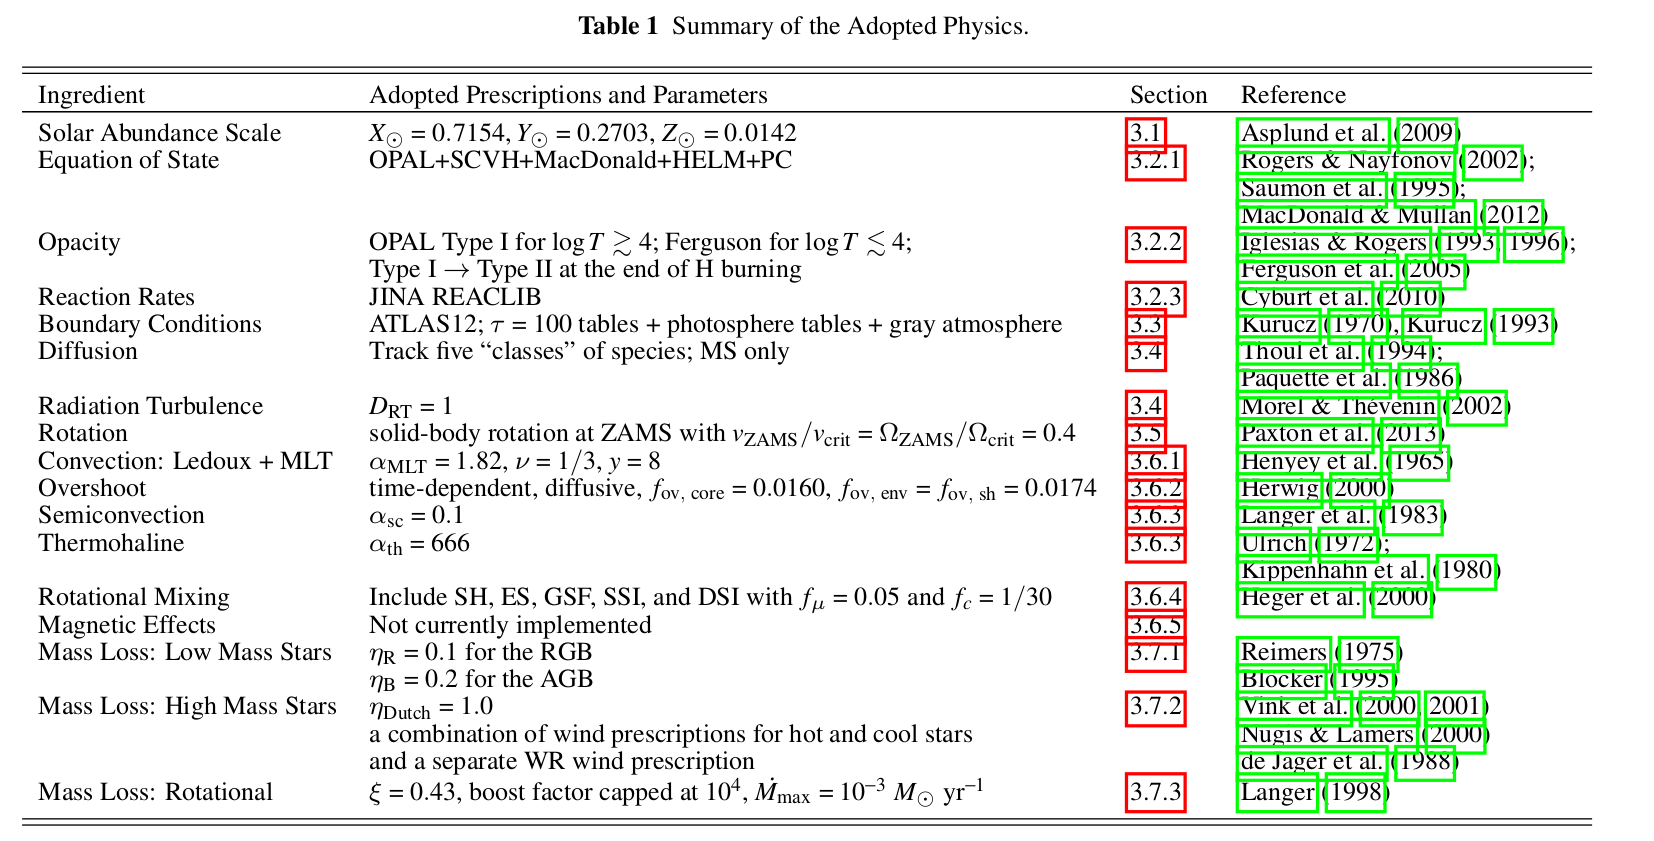
\includegraphics[width=\textwidth]{figs/Choi2016_MIST_table_1.png}
	\caption{Table 1 of C+16. (Purely for reference)}
	\label{fig:table1_C16}
\end{figure}

While C+16 use the protosolar abundances recommended by Asplund et al. 2009 
($Z_{\odot,\mathrm{protosolar}} = 0.0142$), we find, in agreement with the 
solar model discussed by C+16 (Sec. 4), that replicating the bulk properties 
of the Sun at its current age requires adopting fine-tuned protosolar 
abundances.
We insist that our stellar grid reproduce the Sun's radius, luminosity, 
effective temperature to $\lesssim 1\%$ at an age of 4.57 Gyr.
We also insist that our models yield an accurate moment of inertia for the Sun 
(although this is a model-dependent quantity, we can compare our \texttt{MESA} 
profiles with independent models from helioseismology).
For our stellar evolutionary tracks, we adopt the protosolar abundances of
$Y_{\odot,\mathrm{protosolar}} = 0.2612$ and $Z_{\odot,\mathrm{protosolar}} = 
0.0150$, per Table 2 of C+16.\footnote{The tension between the Asplund et al. 
2009 abundances and helioseismology results is to date unresolved, see 
Serenelli 2010 `New results on standard solar models' and Bergemann \& 
Serenelli 2014, `Solar Abundance Problem'.}

In the general case, we then specify the metallicity $\mathrm{[Z/H]=[Fe/H]}$ of 
a given star with respect to $Z_{\odot,\mathrm{protosolar}} = 0.0150$. For 
instance, $\mathrm{[Z/H]=-1}$ corresponds to a metal mass fraction of $0.00150$.
Given $Z$, we find the corresponding hydrogen and helium mass fractions via
\begin{align}
Y_p &= 0.249 
\label{eq:Planck_primordial_He}\\
Y &= Y_p + 
\left(\frac{Y_{\odot,\mathrm{protosolar}}-Y_p}{Z_{\odot,\mathrm{protosolar}}} 
\right) Z \\
X &= 1 - Y - Z,
\end{align}
where the primordial helium abundance $Y_p=0.249$ is adopted from the results 
of the Planck Collaboration (2015).
To find the initial mass fractions of $\mathrm{^1H}$, $\mathrm{^2H}$, 
$\mathrm{^3 He}$, $\mathrm{^4 He}$ (which \texttt{MESA} takes as input), we 
use the isotopic ratios given by Asplund et al. 2009, Table 3.

\subsubsection{Transitions between boundary conditions}
C+16 Sec. 3.3 discusses the various options by which one can constrain the 
temperature and pressure in the outermost cell of a 1D stellar model.
As stated by C+16, the MIST tables (and thus, ours) use a grid 
of 1D plane-parallel atmosphere models computed using ATLAS12 (Kurucz 1970, 
1993). These atmosphere models include molecules that heavily influence the 
opacities of cool dwarfs such as water vapor and titanium monoxide.
With the grid of model atmospheres computed, the standard choice is to set the 
`boundary' at $\tau=2/3$ (the photosphere).
However, the atmospheres of cooler dwarfs are influenced by molecules that are 
not included in \texttt{MESA}'s interior model calculations.
A better choice for cooler dwarfs is thus to set the boundary condition 
at a deeper optical depth, \textit{e.g.}, at $\tau=100$.
C+16 do this by using the \texttt{photosphere\_tables} boundary condition 
for $0.6-10M_\odot$ and the \texttt{tau\_100\_tables} for $0.1-0.3M_\odot$. In 
the intermediate $0.3-0.6M_\odot$, C+16 compute stellar models separately 
using each boundary condition, and then interpolate between them following the 
scheme of Dotter (2016).
We do something similar, but simpler: defined on our desired stellar mass range 
of $0.4-1.2M_\odot$, we say: 
\begin{align}
\mathtt{Boundary\ condition\ table} &=
\begin{cases}
\mathtt{photosphere\_tables} \quad 
&\mathrm{if}\,0.6\leq M_\star/M_\odot<1.2\\
\mathtt{tau\_100\_tables} \quad 
&\mathrm{if}\,0.4\leq M_\star/M_\odot<0.6.
\end{cases}
\end{align}

\textbf{How dependent are our stellar parameters on this latter modeling 
assumption?} We 
show the case of $M_\star=0.5M_\odot$ at $\mathrm{[Z/H]}=-1,-0.5,0,0.5$ in 
Figure FIG, where the y axis is the difference between the two parameters (in 
whatever units are appropriate, and we're asking about L,Teff,R) between using 
the \texttt{photosphere\_tables} and the \texttt{tau\_100\_tables} cases.
%compare plots from grid_2 with grid_production_0. Look at specific difference 
%-- what's the OOM?


\subsection{Comparison to standard solar models}
\label{sec:solar_calibration}
We show our solar calibration in Fig.~\ref{fig:models_near_sun_age}.
`Predicted' values in this plot are: $R_\odot = 
6.957\times10^{10}\,\mathrm{cm}$, $L_\odot = 
3.928\times10^{33}\,\mathrm{erg\,s^{-1}}$, $T_\mathrm{eff,_\odot} = 
5772\,\mathrm{K}$, and $I_\mathrm{tot,\odot} = 
7.0799\times10^{53}\,\mathrm{g\,cm^2} = 
0.0736 M_\odot R_\odot^2$, where $M_\odot = 1.988\times10^{33}\,\mathrm{g}$.
We find the `predicted' solar total moment of inertia by numerically 
integrating the density profile of the standard solar model given by 
Christensen-Dalsgaard et al. 1996.
In Fig.~\ref{fig:models_near_sun_age}, we compute and show 
$I_\mathrm{tot,\star}$ only for our MESA grids because those of the MIST 
project are not published (this was one of the main reasons we opted to make 
our own stellar evolution grids).
The fine-tuned MESA model we use in our grids (solid lines) is `good enough' 
for our purposes: at the Sun's age, we are at $\lesssim 1\%$ agreement with 
predicted values in $R_\star, T_\mathrm{eff,\star}$, and 
$I_\mathrm{\star,tot}$, and $\sim$ 2\% agreement in $L_\star$.
The published `Sun' from C+16's MIST model is further from the expected values 
on all counts\footnote{N.b. the plotted C+16 MIST model is the actual model 
used in the main MIST grids, not the `fine-tuned' solar model discussed in C+16 
Sec. 4. The latter might do better than our MESA-computed model, but is not 
published. We obtain the plotted model by downloading the relevant `EEP track' 
from the 
MIST website, 
\url{http://waps.cfa.harvard.edu/MIST/data/tarballs_v1.0/MIST_v1.0_feh_p0.00_afe_p0.0_vvcrit0.4_EEPS.tar.gz},
and taking the \texttt{00100M.track.eep} model.}.

As a tedious aside, there is no `standard' value for the Sun's moment of 
inertia. The quantity is purely model-determined (a direct measurement would 
require a known torque showing a measurable effect on the sun), and is 
generally computed as 
\begin{equation}
I_{\mathrm{tot,\star}} = \frac{8\pi}{3} \int_0^{R_\star} r^4 \rho(r) dr.
\end{equation}
Thus the density profile completely determines the star's total moment of 
inertia. Various values for $I_\mathrm{tot,\star}$ are quoted in the 
literature without specification of the associated model (e.g., in Allen's 
Astrophysical Quantities (2000), or in Table 19, Ch1 of Yoder's chapter of 
Global Earth Physics (1995)). An older `standard' solar model is Table 28.3 of 
Schwarzschild (1958). Other values are given by M. Bursa et al., Studia 
Geophysica et Geodaftica (1996), Iorio, Solar Physics, 1:47, (2012), and Komm 
et al., Astrophysical J., 586, 650, (2003).
As a heavily-cited and somewhat-recent `standard solar model' (and one that 
`worked', compared to the recent ones that use Asplund abundances), from this 
hodge-podge I selected the model of Christensen-Dalsgaard et al, (1996). 


\begin{figure}[t]
	\centering
	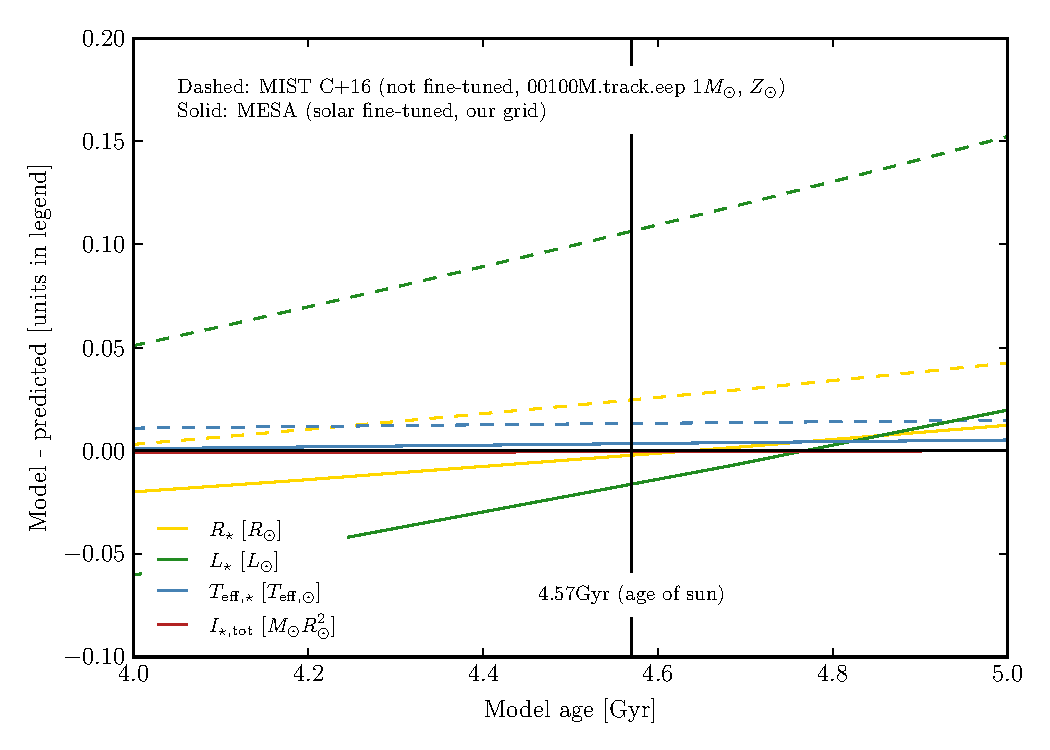
\includegraphics[width=\textwidth]{figs/models_near_sun_age.pdf}
	\caption{Solar calibration (see Sec.~\ref{sec:solar_calibration} for 
	description).}
	\label{fig:models_near_sun_age}
\end{figure}


\subsection{Replicate the MIST profiles}
``But Luke!'', you say, ``you're basically replicating C+16, and 
Fig.~\ref{fig:models_near_sun_age} says you're getting slightly different 
results! How can we be sure that you know what you're doing?''
Answer: by replicating the actual MIST profiles to the best of my ability,
following the description from C+16 and their published \texttt{inlists}.
This gives Fig.~\ref{fig:MESA_MIST_comparison_0.8Msun}.

\begin{figure}[t]
	\centering
  \includegraphics[width=\textwidth]{figs/{MESA_MIST_comparison_0.8Msun}.pdf}
  \caption{Replicating the MIST models (close enough that I'm OK calling them
    `replicated') in the \texttt{Choi\_repl} MESA grids.
  This plot is for $M_\star=0.8M_\odot$, $\mathrm{[Fe/H]=0}$ ($Z=0.015$
  for the \texttt{production\_0} grids, $Z=0.0142$ for \texttt{Choi\_repl}.
  }
	\label{fig:MESA_MIST_comparison_0.8Msun}
\end{figure}


\subsection{The actual grid in $M_\star$ and $Z$}
Satisfied with our sanity checks,
the resulting grid of stellar evolutionary tracks is attached in TABLE, and 
with select models shown in Fig.~\ref{fig:grids}.

\newpage
\clearpage
\begin{figure}[t]
	\thispagestyle{empty}
	\centering
	\includegraphics[width=\textwidth]{figs/grids_2by3.pdf}
	\caption{Stellar evolutionary grids from $0.4-1.2M_\odot$ (more massive 
	means bigger radius and $\sim$smaller convective moment of inertia during 
	MS lifetime).
	The thick black lines are $\mathrm{[Fe/H]}=0$ ($Z\equiv Z_\odot = 0.015$) 
	models, 
	varying over mass.
	The thinner gray lines vary $\mathrm{[Fe/H]}=-1\ \mathrm{to}\ 0.5$, where 
	fainter means lower metallicity. They are shown for $1.1$ and 
	$0.5M_\odot$.		
	}
	\label{fig:grids}
\end{figure}

\end{document}
